% Name: Pythagorean theorem
% Description: A 3-4-5 right triangle with a square on each side, so a² + b² = c² can be seen as area.
% Tags: Pythagorean theorem, right triangle, proof

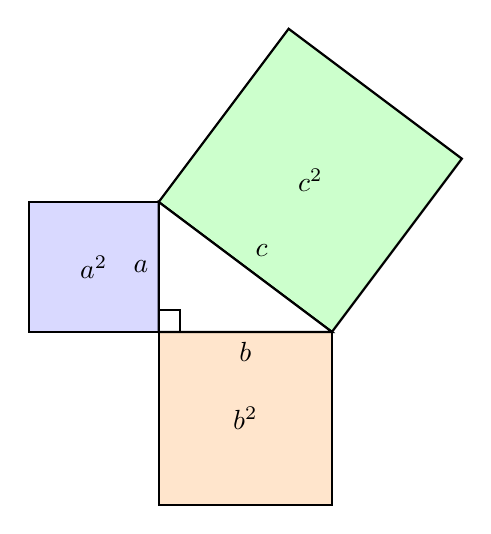
\begin{tikzpicture}[scale=0.55, thick]
  \draw[fill=blue!15] (0,0) -- (0,3) -- (-3,3) -- (-3,0) -- cycle;
  \draw[fill=orange!20] (0,0) -- (4,0) -- (4,-4) -- (0,-4) -- cycle;
  \draw[fill=green!20] (4,0) -- (0,3) -- (3,7) -- (7,4) -- cycle;
  \draw[fill=white] (0,0) -- (4,0) -- (0,3) -- cycle;
  \draw (0,0) rectangle (0.5,0.5);
  \node at (-1.5,1.5) {$a^2$};
  \node at (2,-2) {$b^2$};
  \node at (3.5,3.5) {$c^2$};
  \node[left] at (0,1.5) {$a$};
  \node[below] at (2,0) {$b$};
  \node[above right] at (2,1.5) {$c$};
\end{tikzpicture}
